\documentclass{article}
\usepackage{graphicx}
\usepackage{hyperref}
\usepackage{fontspec}
\setmainfont{Arial}
\setlength{\parindent}{0pt}
\setlength{\parskip}{5pt}
\begin{document}
\section{Users can save money}

Situation now:
\begin{itemize}
\item translate a document to 10 languages
\item each translation costs 1.000€
\item \textbf{cost: 10.000€}
\end{itemize}

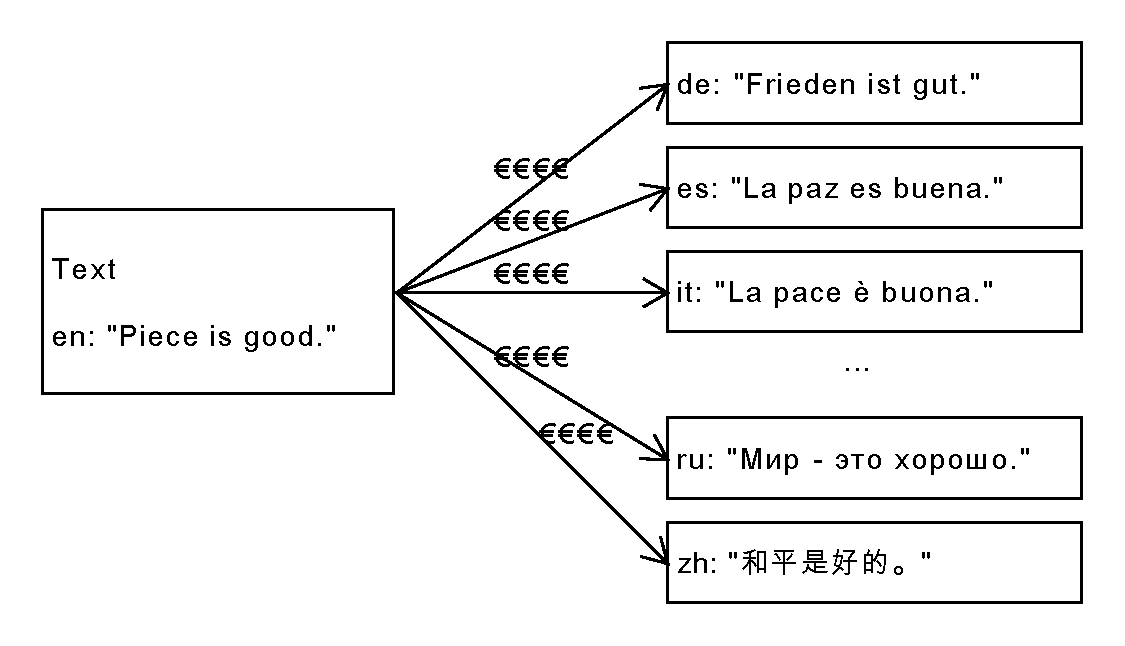
\includegraphics[scale=0.4]{dia/user-view-current-world.pdf}

Goal:
\begin{itemize}
\item encode the document
\item generate 10 language versions
\item encoding costs 2.000€
\item generation doesn't cost anything
\item \textbf{cost: 2.000€}
\end{itemize}

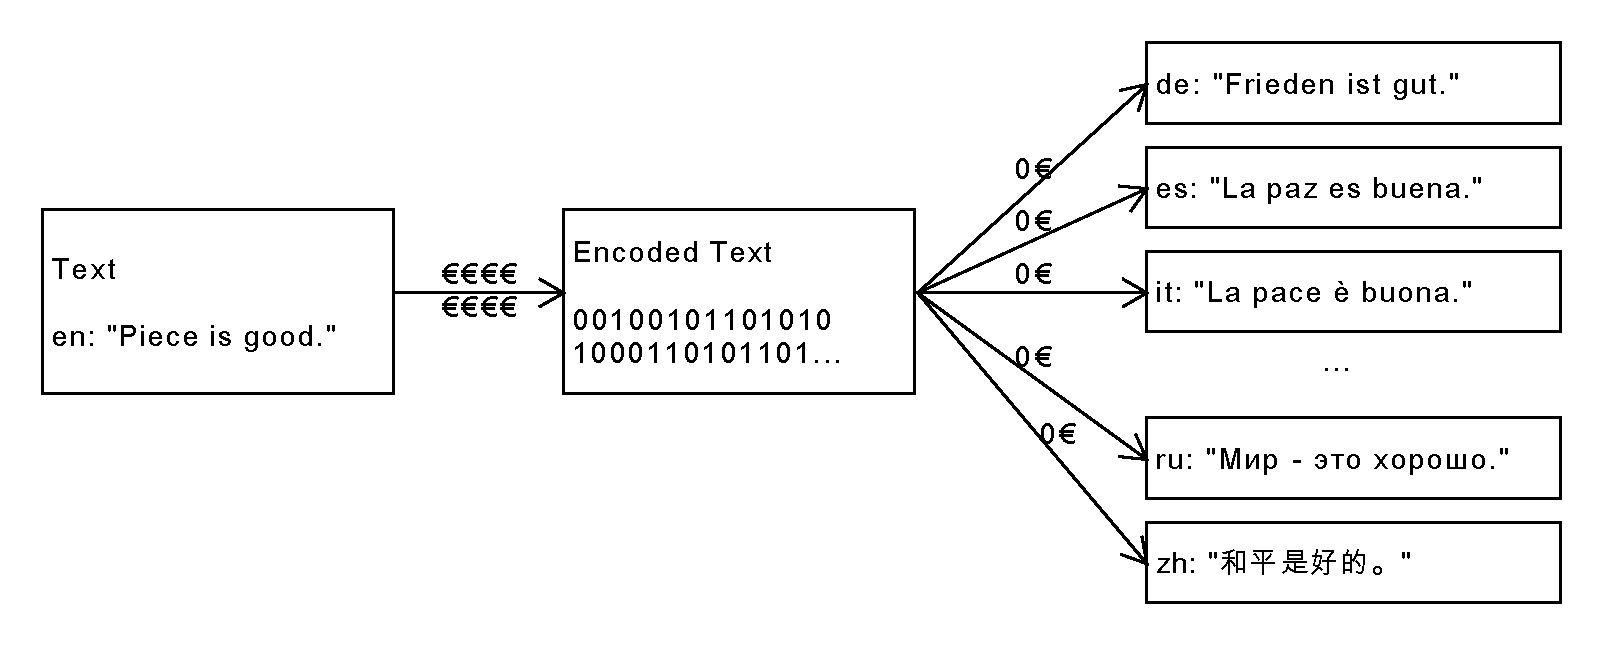
\includegraphics[scale=0.4]{dia/user-view-tokimani.pdf}

Saving: \textbf{8.000€}

\subsection{Some facts about costs}
TODO: how much is spent on translation in the year 2019

TODO: 1.000€ is the cost to translate a document of: 

TODO: in Branchenkennz: xx precent translate to more than k languages.

\section{How}

Existing attempts: full automation

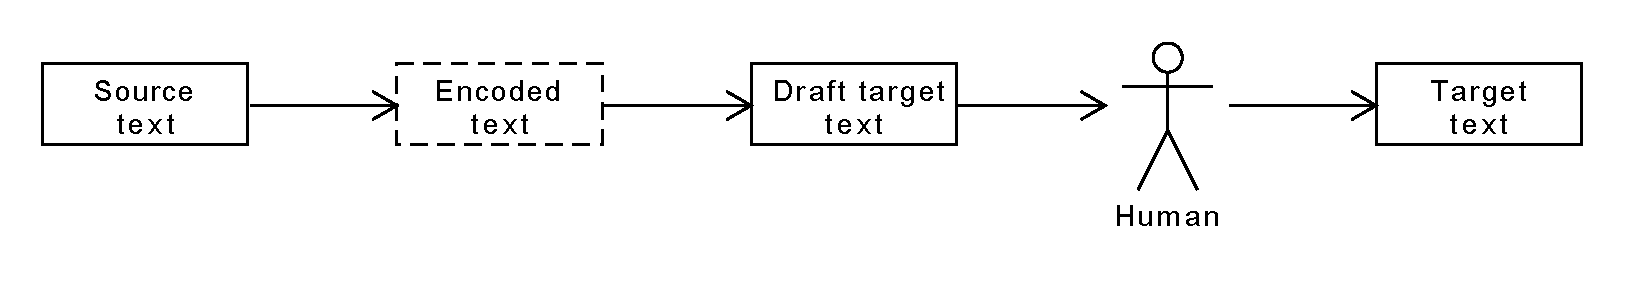
\includegraphics[scale=0.5]{dia/how-current-world.pdf}

Our approach: human in the loop

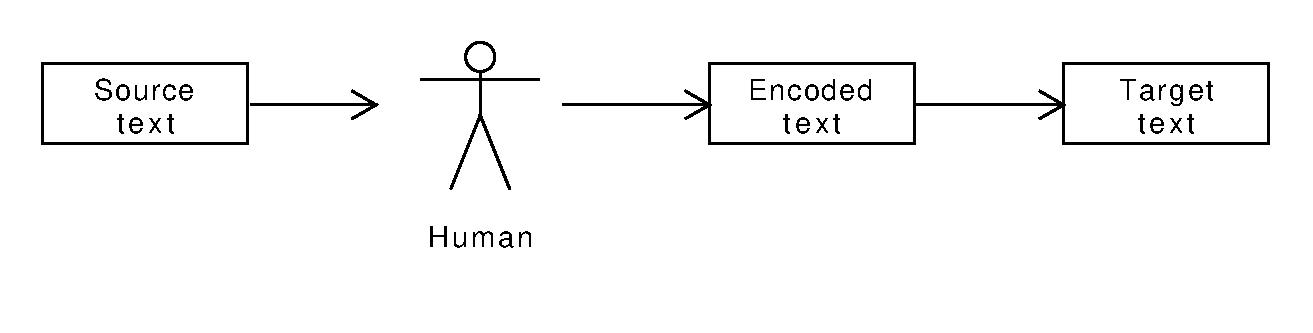
\includegraphics[scale=0.5]{dia/how-tokimani.pdf}

The difference:
\begin{itemize}
\item encoding is made by a human
\item encoded text is human-friendly (for a trained human)
\end{itemize}

\subsection{Why it doesn't exist already}

My hypothesis is: the step "source text to encoded text" can't be automated.

\subsubsection{Fall 1: research}

\begin{itemize}
\item Business has an idea "one source to many targets", likely with the word "automatically".
\item Business ask an university for joint work.
\item Our approach brings nothing scientific new. It leads to no papers. No papers means the end of an academic carier.
\item A researcher subconciously discards our approach even before it comes into mind.
\end{itemize}

\subsubsection{Fall 2: human-first bias}

In related areas, there are successful projects, in which "source text" is restricted by rules, so that "source text" becomes also "encoded text". The keyword is "controlled English".

We go a step further. We declare that being a hauman language is a downside, not a benefit.

\begin{itemize}
\item Having code instead of text is custom-breaking. People don't like changing habits.
\item "Source text" is a front door to a system. A human languages hides complexity elsewhere and gives impresstion that the system is easy.
\end{itemize}


\section{Minimal value product}

To be presented at an user meeting.

\begin{itemize}
\item Audience proposes a phrase conforming to [ASD-STE]
\item The presenter encodes the phrase
\item The system generates English, German, Russian and Spanish
\end{itemize}

\subsection{Milestones}

We rely on:

\begin{itemize}
\item Grammatical Framework [GF], [GF-TALK] and its GF-RGL [GF-RGL] library for multilanguage generation.
\item Lojban [LOJBAN] as inspiration for text encoding.
\end{itemize}

Steps:

\begin{itemize}
\item Done: to learn GF and GF-RGL: describe a small constructed language Toki Pona [TOKIPONA] in GF: [GF-TOKIPONA].
\item Extract examples from "Simplified Technical English" [ASD-STE], encode them in GF-RGL. Use the examples as the ground truth.
\item Learn Lojban, translate the examples to Lojban.
\item Write a converter Lojban to GF-RGL for the examples.
\item Derive CODENAME from Lojban experiments, with a converter from CODENAME to GF-RGL.
\item Create a tool to manage the dictionary.
\item Make Generated texts in English, German, Russian and Spanish good.
\item Profit.
\end{itemize}

References:

\begin{itemize}
\item ASD-STE. ASD Simplified Technical English, \url{http://www.asd-ste100.org/}
\item GF. Grammatical Framework, \url{https://www.grammaticalframework.org/}
\item GF-RGL. GF Resource Grammar Library (RGL), \url{https://github.com/GrammaticalFramework/gf-rgl}
\item GF-TALK. Grammatical Framework: Formalizing the Grammars of the World, \url{https://www.youtube.com/watch?v=x1LFbDQhbso}
\item GF-TOKIPONA. Describe Toki Pona using Grammatical Framework, \url{https://github.com/olpa/gf-tokipona}
\item LOJBAN. Lojban, \url{https://www.lojban.org/}
\item TOKIPONA. Toki Pona, \url{https://tokipona.org/}
\end{itemize}

\end{document}
